\subsection*{Problema 15}

\textbf{Enunciado:} \\
Calcular la integral:
\begin{align*}
\int \dfrac{x^3 - x^2 - 1}{\sqrt{x^2 + 2x + 2}} \, dx
\end{align*}

\textbf{Solución:} \\
Utilizamos el método de coeficientes indeterminados para integrales irracionales (método de Ostrogradski). Planteamos la forma de la solución:
\begin{align*}
\int &\dfrac{x^3 - x^2 - 1}{\sqrt{x^2 + 2x + 2}} \, dx = \\
&(Ax^2 + Bx + C)\sqrt{x^2 + 2x + 2} \\
&+ K \int \dfrac{dx}{\sqrt{x^2 + 2x + 2}}
\end{align*}

Derivamos ambos lados de la ecuación respecto a $x$ para eliminar el signo de integración:
\begin{align*}
\dfrac{x^3 - x^2 - 1}{\sqrt{x^2 + 2x + 2}} &= (2Ax + B)\sqrt{x^2 + 2x + 2} \\
&+ (Ax^2 + Bx + C)\dfrac{2x + 2}{2\sqrt{x^2 + 2x + 2}} \\
&+ \dfrac{K}{\sqrt{x^2 + 2x + 2}}
\end{align*}

Multiplicamos toda la expresión por $\sqrt{x^2 + 2x + 2}$ para simplificar los denominadores:
\begin{align*}
x^3 - x^2 - 1 &= (2Ax + B)(x^2 + 2x + 2) \\
&+ (Ax^2 + Bx + C)(x + 1) + K
\end{align*}

Expandimos los términos del lado derecho:
\begin{align*}
x^3 - x^2 - 1 &= 2Ax^3 + 4Ax^2 + 4Ax \\
&+ Bx^2 + 2Bx + 2B \\
&+ Ax^3 + Ax^2 + Bx^2 \\
&+ Bx + Cx + C + K
\end{align*}

Agrupamos los términos según las potencias de $x$:
\begin{align*}
x^3 - x^2 - 1 &= (3A)x^3 \\
&+ (5A + 2B)x^2 \\
&+ (4A + 3B + C)x \\
&+ (2B + C + K)
\end{align*}

Igualamos los coeficientes de ambos lados de la ecuación polinómica:
\begin{align*}
3A &= 1 \implies A = \dfrac{1}{3} \\
5A + 2B &= -1 \\
4A + 3B + C &= 0 \\
2B + C + K &= -1
\end{align*}

Sustituimos $A = 1/3$ en la segunda ecuación para hallar $B$:
\begin{align*}
5\left(\dfrac{1}{3}\right) + 2B &= -1 \implies 2B = -\dfrac{8}{3} \\
B &= -\dfrac{4}{3}
\end{align*}

Sustituimos $A$ y $B$ en la tercera ecuación para hallar $C$:
\begin{align*}
4\left(\dfrac{1}{3}\right) + 3\left(-\dfrac{4}{3}\right) + C &= 0 \\
\dfrac{4}{3} - 4 + C &= 0 \implies C = \dfrac{8}{3}
\end{align*}

Sustituimos $B$ y $C$ en la cuarta ecuación para hallar $K$:
\begin{align*}
2\left(-\dfrac{4}{3}\right) + \dfrac{8}{3} + K &= -1 \\
-\dfrac{8}{3} + \dfrac{8}{3} + K &= -1 \implies K = -1
\end{align*}

La integral resultante es:
\begin{align*}
\left(\dfrac{1}{3}x^2 - \dfrac{4}{3}x + \dfrac{8}{3}\right)&\sqrt{x^2 + 2x + 2} \\
&- \int \dfrac{dx}{\sqrt{x^2 + 2x + 2}}
\end{align*}

Completando el cuadrado para la integral restante:
\begin{align*}
\int \dfrac{dx}{\sqrt{(x+1)^2 + 1}} = \ln\left|x + 1 + \sqrt{x^2 + 2x + 2}\right|
\end{align*}

Finalmente, la solución general es:
\begin{align*}
\left(\dfrac{x^2 - 4x + 8}{3}\right)&\sqrt{x^2 + 2x + 2} \\
&- \ln\left|x + 1 + \sqrt{x^2 + 2x + 2}\right| + C
\end{align*}

\begin{figure}[H]
	\centering
	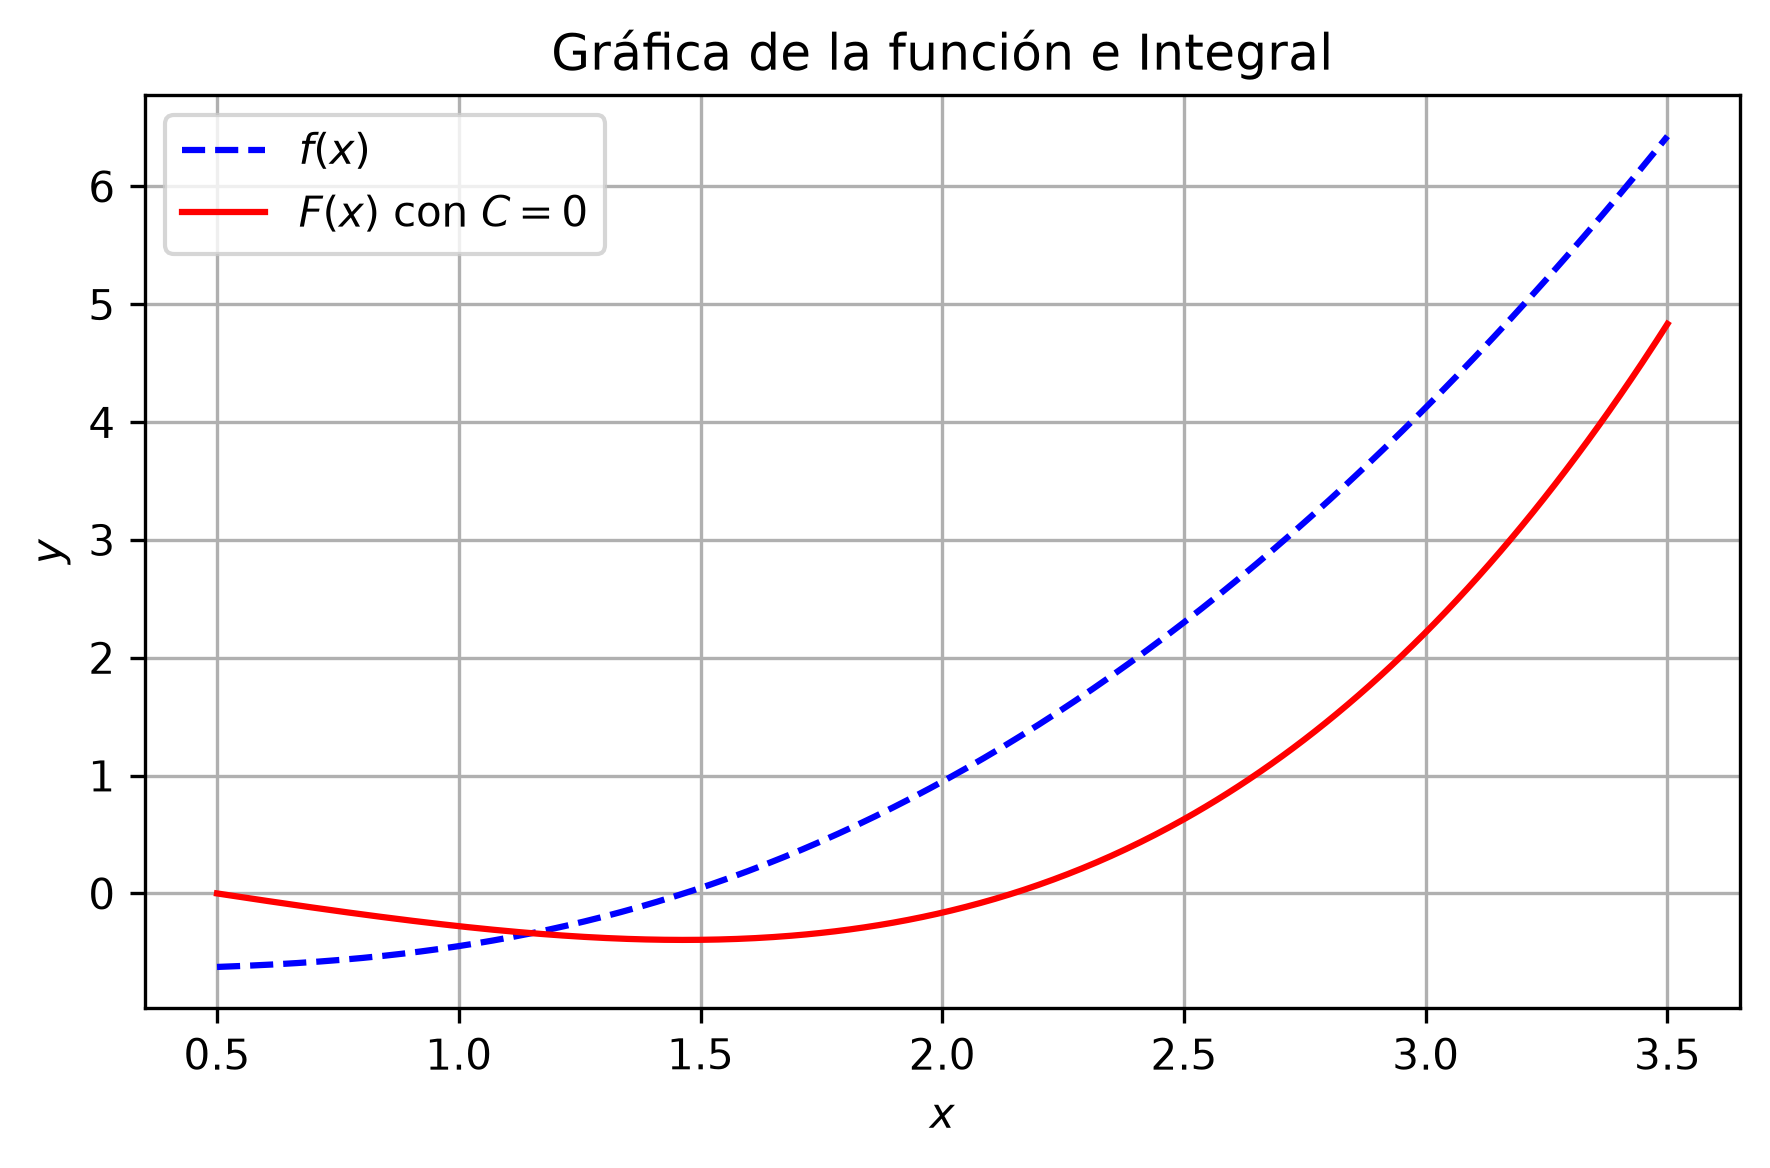
\includegraphics[width=\columnwidth]{semana_05/graficas/SEM05_P15_grafica.png}
	\caption{Representación gráfica de $f(x)$ y su antiderivada $F(x)$ evaluada para la constante de integración $C = 0$ (Problema 15).}
	\label{fig:problema15}
\end{figure}
